\documentclass[12pt,a4paper]{article}
\usepackage[utf8]{inputenc}
\usepackage[brazil]{babel}
\usepackage{graphicx}
\usepackage{amssymb, amsfonts, amsmath}
\usepackage{float}
\usepackage{enumerate}
\usepackage[top=1.5cm, bottom=1.5cm, left=1.25cm, right=1.25cm]{geometry}

\begin{document}
\pagestyle{empty}

\begin{center}
  \begin{tabular}{ccc}
    \begin{tabular}{c}
      \includegraphics[scale=0.25]{../../biblioteca/imagem/brasao-de-armas-brasil} \\
    \end{tabular} & 
    \begin{tabular}{c}
      Ministério da Educação \\
      Universidade Federal dos Vales do Jequitinhonha e Mucuri \\
      Faculdade de Ciências Sociais, Aplicadas e Exatas - FACSAE \\
      Departamento de Ciências Exatas - DCEX \\
      Disciplina: Matemática I \quad Semestre: 2020/1\\
      Prof. Me. Luiz C. M. de Aquino\\
    \end{tabular} &
    \begin{tabular}{c}
      \includegraphics[scale=0.25]{../../biblioteca/imagem/logo-ufvjm} \\
    \end{tabular}
  \end{tabular}
\end{center}

\begin{center}
  \textbf{Lista III}
\end{center}

\begin{enumerate}
  \item Determine o domínio das funções definidas abaixo.
  \begin{enumerate}
    \item $f(x) = \sqrt{x - 2}$.
    \item $g(t) = \dfrac{\sqrt{2t^2 - 5t + 2} - 1}{1 - 2t}$.
    \item $h(u) = \dfrac{\sqrt{2u - u^2} + \sqrt{u^2 - 4u + 3}}{u - 4}$.
    \item $i(s) = \dfrac{\sqrt{s + 2} - \sqrt{3 - s}}{s^2 - 9}$.
  \end{enumerate}
  
  \item Os gráficos das funções $f$ e $g$ estão ilustrados abaixo. Determine o ponto de interseção entre esses gráficos.
  
    \begin{figure}[H]
     \centering
     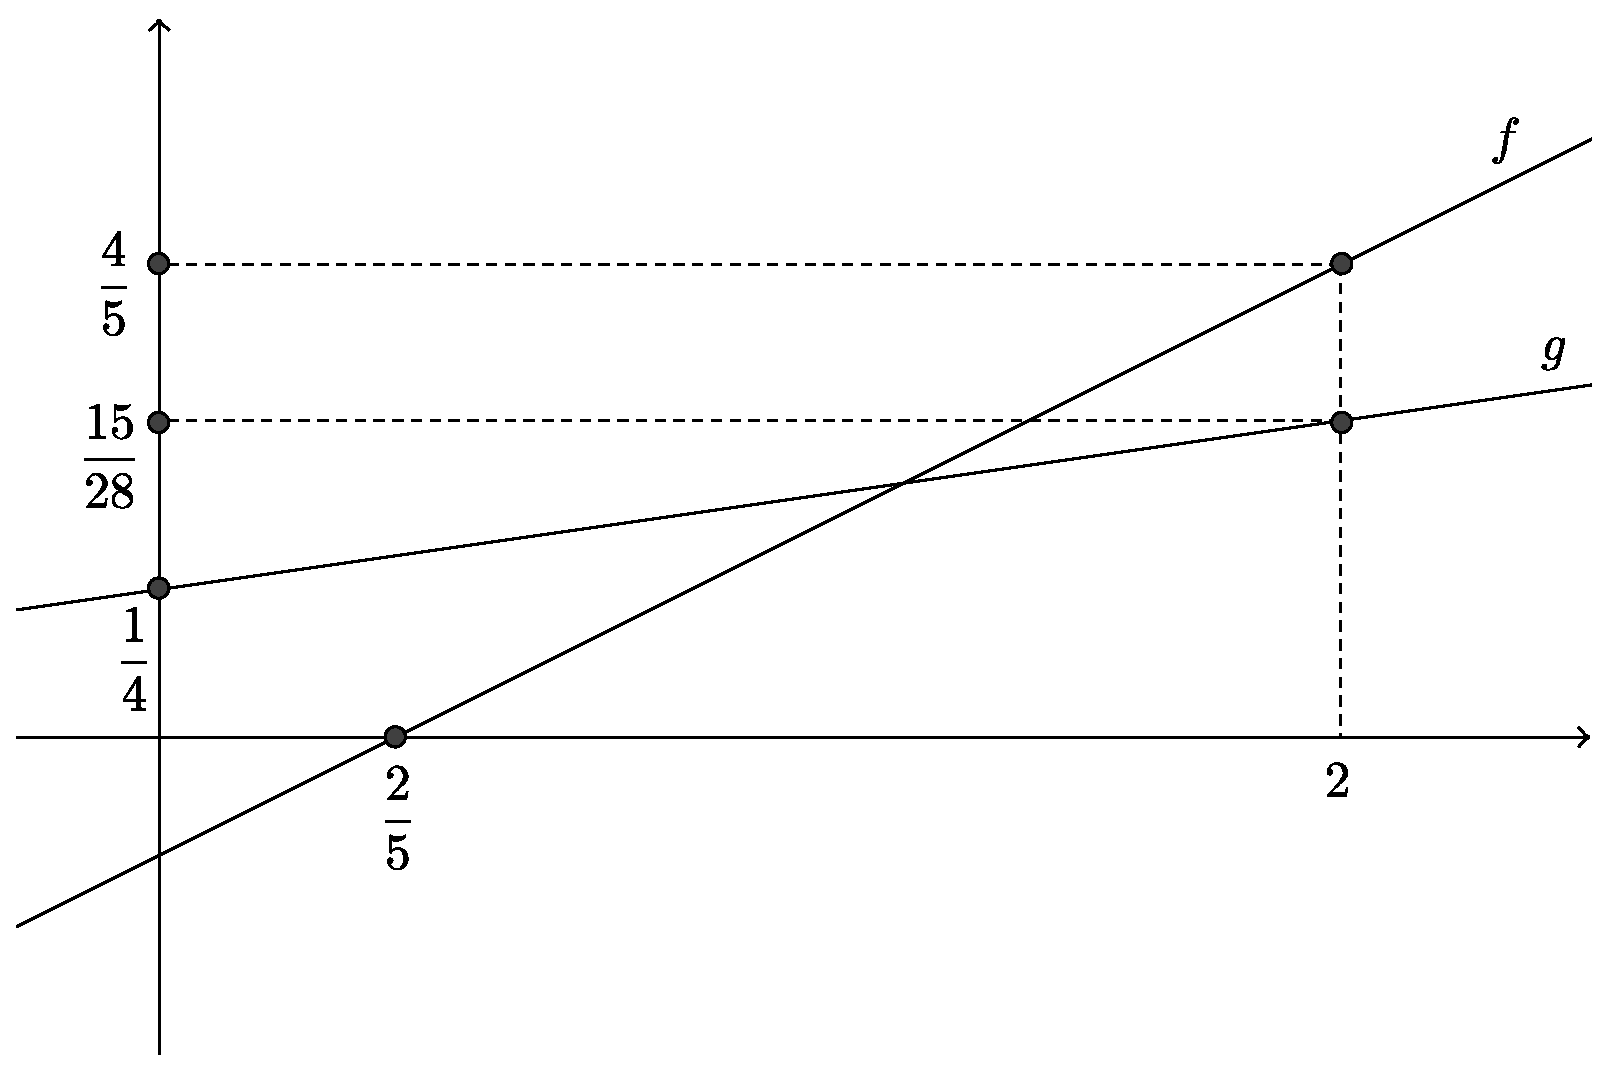
\includegraphics[scale=0.4]{figura/grafico-intersecao-de-retas.eps}
    \end{figure}
  
  \item Uma empresa aluga veículos cobrando uma taxa fixa de R\$ 20,00 e mais
    R\$ 0,40 por quilômetro percorrido. Sabendo-se que uma pessoa pagou
    R\$ 56,80 após um aluguel nessa empresa, quantos quilômetros essa pessoa
    percorreu com o veículo alugado?

  \item Duas empresas prestam serviço de entrega. Considere que $A(t)$ é o valor
    cobrado pela empresa $A$, supondo que $t$ quilômetros foram percorridos para
    efetuar a entrega. Já $B(t)$ é o valor cobrado pela empresa $B$, supondo que
    $t$ quilômetros foram percorridos para efetuar a entrega. A figura a seguir
    ilustra o gráfico dos valores cobrados conforme a quantidade de quilômetros
    percorridos. Supondo que os valores $A(t)$ e $B(t)$ se comportam de maneira
    linear, responda aos quesitos abaixo.
  
  \begin{figure}[H]
    \centering
    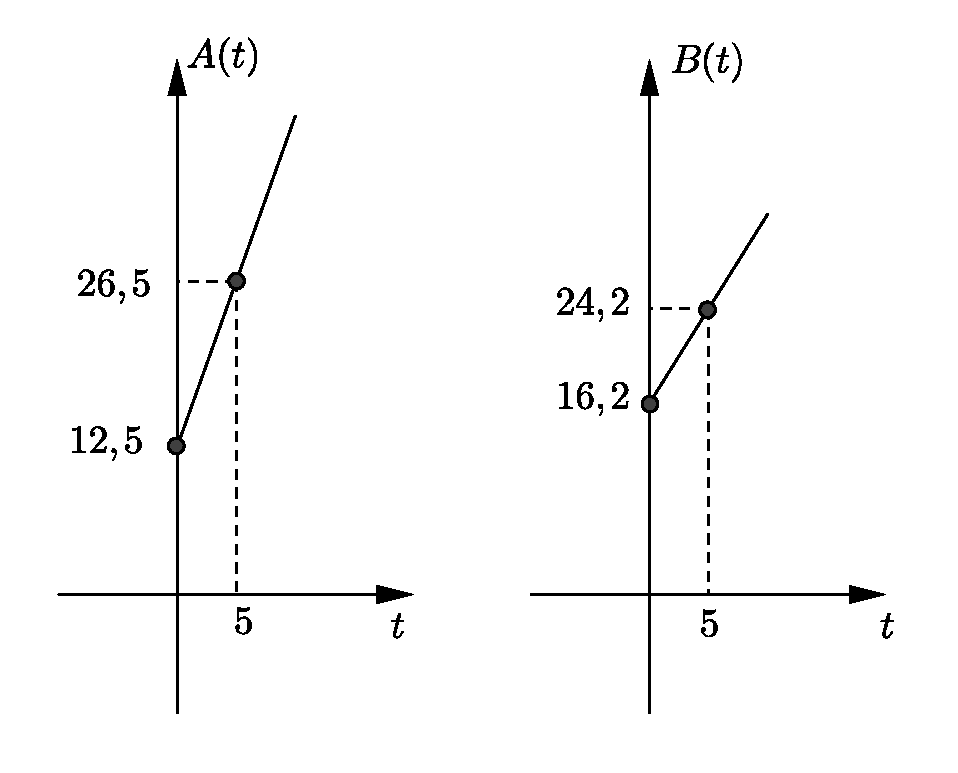
\includegraphics[scale=0.5]{figura/grafico-duas-empresas.eps}
  \end{figure}
  
  \begin{enumerate}
    \item Calcule o valor $A(4)$ e $B(4)$.
    \item Em cada empresa, se R\$ 40,00 for o valor cobrado por uma entrega, então quantos quilômetros foram percorridos para efetuá-la?
    \item A partir de quantos quilômetros o valor $B(t)$ é menor do que $A(t)$?
  \end{enumerate}

  \item Determine os pontos de interseção entre os gráficos das funções definidas por 
  $f(x) = 3x^2 + 12x - 7$ e $g(x) = -4x + 5$.
  
  \item Considere que $f$ é uma função polinomial do 2° grau, cujo o gráfico está
  ilustrado abaixo. Determine os pontos de interseção entre esse gráfico e o eixo $x$.

  \begin{figure}[H]
   \centering
   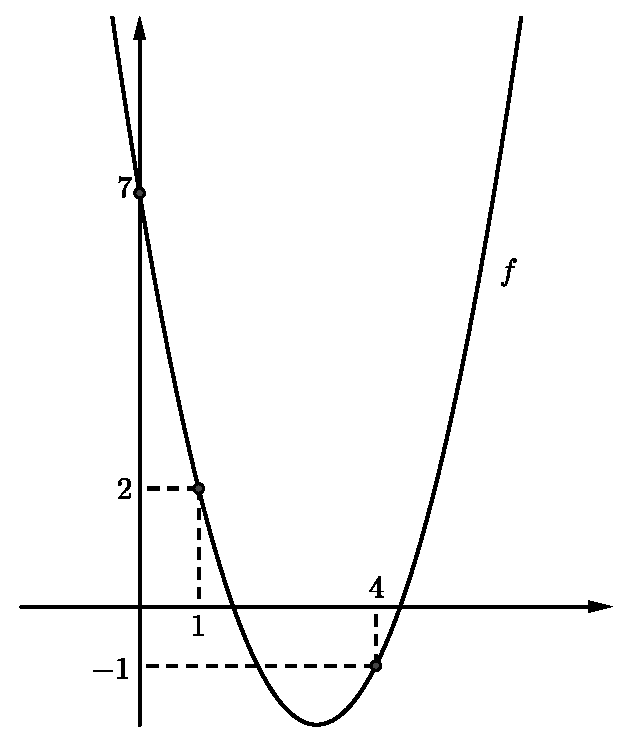
\includegraphics[scale=0.625]{figura/grafico-funcao-polinomio-segundo-grau.eps}
  \end{figure}
  
  \item O dono de uma lanchonete cobra R\$ 9,00 por uma pizza, sendo que seu custo
    para produzi-la é R\$ 4,00. Ele deseja aumentar o valor da pizza, mas antes disso
    decidiu analisar seu histórico de vendas. Ele percebeu que ao cobrar $x$ reais
    por uma pizza, ele vendia aproximadamente $20 - x$ pizzas por dia. Nessas condições,
    qual deve ser o aumento para que diariamente ele tenha lucro máximo na
    venda das pizzas?
  
\end{enumerate}

\end{document}